\section{Return patterns around reconstitution}
\subsection{Lower recent averages without a monotonic disappearance}

Table~\ref{tab:returns} reports the announcement, implementation and total-window return means. Additions have positive total-window means in every period, but their magnitudes vary sharply. The first block is exceptional at 8.52\%. The second falls to 0.25\%, the third rises to 2.85\%, and the latest is 1.50\%. This sequence is compatible with an attenuation from the unusually high early observations, but it is not a monotonic decline toward zero.

\begin{table}[!htbp]
\centering
\caption{Market adjusted returns around index changes}\label{tab:returns}
\small
\setlength{\tabcolsep}{5pt}
\begin{tabular}{llrrrrrlr}
\toprule
Type & Period & $N$ & $G$ & AD & ED & Total & 95\% interval & $p$ \\
\midrule
Addition & 2007--2011 & 33 & 9 & 0.96 & 1.16 & 8.52 & [2.46, 14.74] & 0.027 \\
Addition & 2012--2016 & 54 & 10 & 1.87 & -0.73 & 0.25 & [-3.73, 5.30] & 0.908 \\
Addition & 2017--2021 & 82 & 10 & -0.16 & 0.38 & 2.85 & [1.26, 5.20] & 0.005 \\
Addition & 2022--2026 & 87 & 9 & 1.20 & -0.09 & 1.50 & [-0.10, 3.22] & 0.062 \\
Deletion & 2007--2011 & 33 & 9 & -0.77 & -0.09 & -6.16 & [-11.41, -2.10] & 0.007 \\
Deletion & 2012--2016 & 46 & 10 & -1.71 & -0.85 & -2.47 & [-14.42, 3.60] & 0.522 \\
Deletion & 2017--2021 & 61 & 10 & -2.09 & 0.89 & -0.43 & [-3.43, 3.02] & 0.759 \\
Deletion & 2022--2026 & 75 & 9 & -0.71 & -1.23 & -1.53 & [-4.24, 0.89] & 0.279 \\
\bottomrule
\end{tabular}
\begin{minipage}{\linewidth}\footnotesize\vspace{5pt}
Returns are percentages. AD denotes CAR $[AD-1,AD+1]$, ED denotes CAR $[ED-1,ED+1]$, and Total denotes CAR $[AD-1,ED+1]$, where AD is the recorded announcement trading date and ED the effective trading date. The benchmark is OMXSBGI. Means weight events equally. $N$ and $G$ are event and review counts for Total; AD and ED use their own complete cases. Intervals and two-sided $p$-values for Total use the inherited restricted wild cluster bootstrap with 9,999 draws, Webb weights below 12 clusters and Rademacher weights otherwise. These are pointwise, exploratory intervals. No stars are used. Source: effect/tabell1\_lang.csv, panel A/B.
\end{minipage}
\end{table}


Announcement-window means are substantially smaller than the first period's total-window mean. Implementation-window means are close to zero in the latest block: -0.09\% for additions and -1.23\% for deletions, with wide intervals in the underlying outputs. A small implementation-window return does not imply an absence of benchmark-related trading. If investors anticipate the reconstitution, or if liquidity supply absorbs trading near implementation, any associated price movement may occur elsewhere. Conversely, a return between announcement and implementation can also reflect unrelated information over that interval.

Deletion means are -6.16\%, -2.47\%, -0.43\% and -1.53\% across the four blocks. Their uncertainty is large, especially in 2012--2016. In that block, the event-weighted mean and equal-review mean differ considerably, illustrating why a larger event count cannot replace balanced independent review information. The economically relevant statement is that deletion returns are less precisely resolved, rather than that the deletion channel is absent.

\begin{figure}[!htbp]\centering
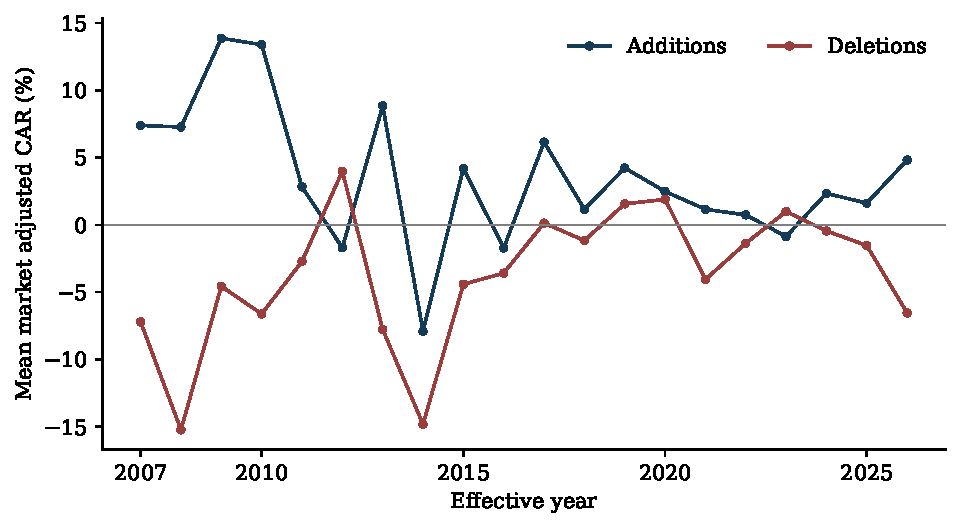
\includegraphics[width=.94\linewidth]{figures/annual_returns.pdf}
\caption{Annual mean market-adjusted returns. Each point is the event-weighted CAR $[AD-1,ED+1]$ for additions or deletions in an effective calendar year. The final point covers only the first 2026 review. Lines connect descriptive annual averages and are not fitted trends. Some years contain very few usable events; the figure carries no annual inferential bands. Source: effect/effect\_by\_year.csv.}\label{fig:annual}
\end{figure}

Table~\ref{tab:contrasts} separates three different time-comparison questions. The latest-minus-earliest addition contrast is -7.03 percentage points, with a pointwise bootstrap interval of [-13.10, -1.10]. The corresponding deletion contrast is +4.62 percentage points: deletions become less negative relative to the first block. Both contrasts concern the endpoints of this sample. Neither establishes a gradual annual decline, and their nominal significance weakens under the ten-test audit correction.

\begin{table}[!htbp]
\centering
\caption{Changes in the event window return}\label{tab:contrasts}
\small
\setlength{\tabcolsep}{5pt}
\begin{tabular}{lllrr}
\toprule
Type & Contrast & Estimate & 95\% interval & $p$ \\
\midrule
Addition & Latest minus earliest & -7.03 & [-13.10, -1.10] & 0.029 \\
Addition & Latest minus preceding & -1.35 & [-3.88, 0.98] & 0.250 \\
Addition & Later minus earlier decade & -1.24 & [-5.26, 2.54] & 0.502 \\
Addition & Linear trend per year & -0.28 & [-0.64, 0.08] & 0.117 \\
Deletion & Latest minus earliest & 4.62 & [0.25, 9.81] & 0.039 \\
Deletion & Latest minus preceding & -1.10 & [-5.11, 2.70] & 0.564 \\
Deletion & Later minus earlier decade & 2.97 & [-2.94, 8.60] & 0.328 \\
Deletion & Linear trend per year & 0.19 & [-0.29, 0.64] & 0.400 \\
\bottomrule
\end{tabular}
\begin{minipage}{\linewidth}\footnotesize\vspace{5pt}
The outcome is CAR $[AD-1,ED+1]$. Differences are percentage points; the linear trend is percentage points per calendar year. Earliest, preceding, and latest periods are 2007--2011, 2017--2021, and 2022--2026. Decades are 2007--2016 and 2017--2026. Restricted wild bootstrap inference clusters by review cycle, using 9,999 draws. A difference of significance levels across periods is not a test of a difference. Source: effect/tabell1\_lang.csv, panel D.
\end{minipage}
\end{table}


The change from 2017--2021 to 2022--2026 is much less precisely estimated. For additions it is -1.35 percentage points, with an interval spanning zero. The later-minus-earlier decade contrast is -1.24 percentage points and is also imprecise. The linear addition trend is approximately -0.28 percentage points per year, again with a bootstrap interval including zero. These estimates do not contradict the large earliest-to-latest difference; they show that the shape and timing of the attenuation are unresolved by a single summary coefficient.

The repository contains a previously selected breakpoint around June 2010. Because that timing emerged in earlier analysis of the same return history, a conventional test that subsequently treats it as fixed understates the uncertainty associated with searching for the break. We do not promote that breakpoint to a new identified regime change. The annual plot and the full set of period contrasts provide the descriptive evidence without implying a verified event behind the apparent change.

\subsection{Recent returns and the meaning of an insignificant estimate}

Pooling 2017--2026 yields a mean addition CAR of 2.15\%, with a 95\% wild-bootstrap interval of [1.01\%, 3.39\%]. This average covers 169 additions over 19 review cycles. The corresponding deletion mean is -1.04\%, with an interval of approximately [-2.88\%, 0.90\%], over 136 deletions and 19 cycles. The sign and precision differ, but we do not infer an addition-deletion asymmetry from separate significance decisions; such an asymmetry would require a direct contrast on a consistent estimand.

The final five-year addition block contains 87 observations over nine reviews. Its 1.50\% estimate has a bootstrap interval spanning zero and returns above 3\%. The archived analytical MDE is approximately 2.35 percentage points. These facts make a null result weak evidence for disappearance. At the audit's one-percentage-point margin, the 90\% analytical interval is [0.13\%, 2.87\%], so it does not lie inside the equivalence band. Deletions also fail equivalence, with an interval of [-3.62\%, 0.55\%].

The interval for the latest addition mean cannot be interpreted as a confidence interval for a causal membership premium. It is uncertainty about the market-adjusted mean among the observed events under the maintained inference model. The economic interpretation is narrower but still useful: the recent sample cannot distinguish a small effect from a positive association of meaningful magnitude. A statement that the effect has ``disappeared'' would omit precisely the uncertainty that matters for that question.

\subsection{Composition and comparison securities}

Table~\ref{tab:composition} reports the observable-composition adjustment. For additions, the latest-period estimate is 1.59\% without controls on the common sample and 1.60\% with controls. The early-period values are 8.97\% and 10.12\%, respectively. In this particular linear adjustment, the four covariates do not explain away the early-to-late difference. That finding is descriptive: the variables may not capture the relevant selection process, their construction uses nearby price information, and some are themselves related to anticipated membership.

\begin{table}[!htbp]
\centering
\caption{Composition adjustment on a common event sample}\label{tab:composition}
\small
\setlength{\tabcolsep}{5pt}
\begin{tabular}{llrrl}
\toprule
Type & Period & Unadjusted & Adjusted & Adjusted CR1 interval \\
\midrule
Addition & 2007--11 & 8.97 & 10.12 & [5.09, 15.16] \\
Addition & 2012--16 & 0.74 & 0.55 & [-3.01, 4.11] \\
Addition & 2017--21 & 2.64 & 2.33 & [0.38, 4.29] \\
Addition & 2022--26 & 1.59 & 1.60 & [0.68, 2.53] \\
Deletion & 2007--11 & -5.66 & -6.23 & [-11.03, -1.43] \\
Deletion & 2012--16 & -1.37 & -1.42 & [-7.61, 4.76] \\
Deletion & 2017--21 & -0.77 & -0.29 & [-3.35, 2.77] \\
Deletion & 2022--26 & -1.83 & -1.95 & [-4.02, 0.12] \\
\bottomrule
\end{tabular}
\begin{minipage}{\linewidth}\footnotesize\vspace{5pt}
Period intercepts from CAR $[AD-1,ED+1]$ regressions. Both columns use the same complete-case sample: 237 additions or 185 deletions. Adjusted estimates control for centered abnormal turnover, relative size, residual return variance and analyst coverage. The columns are not a causal decomposition. Intervals are analytical CR1 review-clustered intervals using $t_{G-1}$; unstable inverted bootstrap intervals from auxiliary sparse specifications are not used here. Source: composition/tabell2\_tabell4.csv, table 2.
\end{minipage}
\end{table}


For deletions, the common-sample latest-period estimates are -1.83\% without controls and -1.95\% with controls. Differences between these numbers and the full return table partly reflect complete-case selection. The adjusted regression contains 185 deletions, compared with 215 in the main return table. The separate common-sample column prevents that reduction from being attributed entirely to economic controls.

The size-screened comparison regression offers another descriptive perspective. The later-decade addition coefficient is 1.53 percentage points, with a bootstrap interval of [0.36, 2.68]. Restricting comparison securities to the main market produces 1.39 percentage points, with an interval of [0.12, 2.60]. The corresponding later-decade deletion coefficient is -1.40 percentage points, with an interval reaching slightly above zero. Table~\ref{tab:comparators} reports the main comparison results and counts.

\begin{table}[!htbp]
\centering
\caption{Returns relative to size screened comparison securities}\label{tab:comparators}
\small
\setlength{\tabcolsep}{5pt}
\begin{tabular}{llrrrlr}
\toprule
Type & Period & Events & Controls & Coefficient & 95\% interval & $p$ \\
\midrule
Addition & 2007--2016 & 78 & 787 & 3.90 & [0.10, 8.07] & 0.046 \\
Addition & 2017--2026 & 159 & 1609 & 1.53 & [0.36, 2.68] & 0.015 \\
Deletion & 2007--2016 & 68 & 415 & -3.24 & [-9.27, 1.17] & 0.210 \\
Deletion & 2017--2026 & 130 & 833 & -1.40 & [-2.75, 0.03] & 0.053 \\
\bottomrule
\end{tabular}
\begin{minipage}{\linewidth}\footnotesize\vspace{5pt}
The coefficient is on an event indicator in a regression of CAR $[AD-1,ED+1]$ on that indicator, pre-announcement returns, log market capitalization and review fixed effects. Comparison observations are security-review observations, not unique firms. The inherited size screens do not reconstruct the Nasdaq inclusion threshold and are not a regression discontinuity design. The pre-return control includes AD-1, which also enters the outcome; this overlap is an additional reason to treat the coefficients as descriptive adjustments. Intervals and $p$-values use 9,999 restricted wild cluster draws by review. Source: near\_additions/near\_additions\_results.csv.
\end{minipage}
\end{table}


These results show that the later addition association is not mechanically identical to the average return of the available comparison group. They do not show that a particular fraction of the raw CAR is caused by index membership. The raw and conditional estimates use different samples, weights and assumptions. Subtracting one from the other would not isolate a causal selection component. The lack of a reconstructed Nasdaq assignment boundary and the overlapping pre-return control remain substantive limitations.

\FloatBarrier
